\documentclass[conference]{IEEEtran}
% Compile with pdfLaTeX (Overleaf default). Figures are in ./figures.

\usepackage[T1]{fontenc}
\usepackage{graphicx}
\usepackage{booktabs}
\usepackage{tabularx}
\usepackage{array}
\usepackage{tikz}
\usepackage{xcolor}
\usepackage{url}
\usepackage[hidelinks]{hyperref}

\newcommand{\dom}[1]{\texttt{#1}}
\newcommand{\say}[1]{``\emph{#1}''}

\begin{document}

\title{VoiceGuard: Making Authentication Attacks\\Audible to Screen-Reader Users}

\author{
\IEEEauthorblockN{Qazi Muhammad Waiz (28982), Haris Shibli (28988), Abdullah Feroz (29219)}
\IEEEauthorblockA{Human-Computer Interaction, Institute of Business Administration (IBA), Karachi\\
Fall 2026}
}

\maketitle

\begin{abstract}
Screen-reader users hear sign-in security instead of seeing it, and three attacks exploit what the audio leaves out: look-alike domains that sound identical, an attacker's push notification that replaces the user's own, and push spam that wears the user down. \emph{Broken Access} (WWW~'25) diagnosed these gaps but built no fixes. We present \textbf{VoiceGuard}, a screen-reader-aware security layer that makes each attack audible. It names the exact difference between a fake and a real domain in the NATO alphabet, keeps every push visible with a spoken code word that ties it to the user's own sign-in, locks approval under push spam, sizes expiry windows to speech time, and lets users answer a push by voice. In an automated evaluation using the paper's own similarity metric, VoiceGuard detected 99.6\% of 1,114 generated look-alike domains with no false alarms on 85 real sites. The paper's example pair sounds 100\% identical through a screen reader today and 60.4\% similar with VoiceGuard. An ablation shows that the spoken code word is the only defence once an attacker copies the victim's device, and the approval lock the only defence under spam. In scripted keyboard-only sessions in a real browser, attacks succeeded 3 of 4 times under today's behaviour and 0 of 4 with VoiceGuard, while legitimate sign-ins still succeeded. In a pilot session, a blind participant using today's behaviour approved an attacker's push by voice after six spam requests. The core problem is audibility, not detection.
\end{abstract}

\begin{IEEEkeywords}
accessibility, screen readers, authentication, phishing, push notifications, MFA fatigue, usable security
\end{IEEEkeywords}

%======================================================================
\section{Introduction}

Sign-in security now depends on details people check by eye. A sighted user can spot a misspelled domain or notice two sign-in prompts on a phone. A screen-reader user hears these details instead, and the audio often drops them. About 43 million people are blind and 295 million have moderate-to-severe visual impairment; many sign in through NVDA, JAWS, VoiceOver or TalkBack.

Akanda, Mahdad and Saxena's \emph{Broken Access}~\cite{brokenaccess} measured this gap. Using their AWARE framework, they found that every deployed two-factor and passwordless method had an accessibility gap, a security gap, or both. Their discussion recommends fixes in one paragraph: a phishing detector inside the screen reader, announcing the requesting service, a detector for repeated notifications, and expiry windows long enough for speech. They do not build or test any of them.

We build and test them. Our premise is that all three attacks we target exploit the \emph{voice channel}: what is spoken, when, and what is left out. VoiceGuard therefore fixes what the user hears, not only what the system detects.

\textbf{Objective.} The objective of this experiment is to build VoiceGuard and test whether it makes phishing, concurrent-login and push-fatigue attacks detectable by ear for screen-reader users, without making normal sign-in harder. We ask five research questions:
\begin{itemize}
\item \textbf{RQ1:} Does VoiceGuard reduce phishing success?
\item \textbf{RQ2:} Does it reduce approval of a concurrent attacker push?
\item \textbf{RQ3:} Does it reduce acceptance of push spam (fatigue)?
\item \textbf{RQ4:} What does the protection cost in usability (sign-in success and time, SUS, NASA-TLX)?
\item \textbf{RQ5:} Does it make look-alike domains \emph{audibly} different, measured with AWARE's similarity metric?
\end{itemize}

Our contributions are:
\begin{enumerate}
\item \textbf{VoiceGuard}, with a domain guard for phishing and a push guard for concurrent-login and push-fatigue attacks, plus voice answering on the phone.
\item \textbf{A study environment}: simulated computer and phone, an attacker console, and an experimenter console for counterbalanced, auto-scored sessions.
\item \textbf{An automated evaluation} that reproduces the paper's 100\% similarity finding and measures VoiceGuard on 1,114 look-alike domains.
\item \textbf{An ablation} showing which push-guard component closes which gap.
\item \textbf{End-to-end sessions} in a real browser, driven keyboard-only by a scripted user, in both conditions.
\item \textbf{A pilot session with a blind participant}, and the practical lessons it produced.
\end{enumerate}

%======================================================================
\section{Background and Related Work}

\textbf{AWARE and \emph{Broken Access}.} AWARE~\cite{brokenaccess} records what a screen reader says, transcribes it, and scores how much information survives using TF-IDF cosine similarity. It then simulates attacks and re-runs the check after fixes. Across six screen readers and twelve authentication methods it found 100\% audio similarity between \dom{bankofamerica.com} and \dom{bankoffamerica.com}; that the attacker's push replaces the victim's in Google Push (VoiceOver, TalkBack) and Duo Push; and that comprehension collapses at faster speech rates (37\% at the default rate, 0\% at 80\% and above). It also cites prior work in which only 5\% of users noticed a concurrent-login attack. We reuse its similarity metric so our numbers compare directly.

\textbf{Look-alike domains.} Homograph attacks swap letters for visually identical Unicode characters~\cite{homograph}, typosquatting registers near-misspellings~\cite{typosquat}, and combosquatting adds words such as ``login'' to a brand~\cite{combosquat}. Detection is well studied, using edit distance, confusable tables such as Unicode TR39~\cite{tr39} and Punycode decoding~\cite{punycode}. VoiceGuard uses these standard techniques; its contribution is how the result is \emph{spoken}.

\textbf{Push abuse.} Push-fatigue (``MFA bombing'') attacks send repeated approval requests until one is accepted. Number matching is the main deployed defence; \emph{Broken Access} found it can be blocked or shown with malicious options, with no screen-reader warning. VoiceGuard's spoken code word applies the same idea to the audio channel.

%======================================================================
\section{Threat Model and Problems}

The victim signs in with a password on a computer and approves a push on a phone, the PC-plus-smartphone setting used by 49.2\% of screen-reader users~\cite{brokenaccess}. The attacker knows the victim's bank, can register domains, send email and start sign-ins once it has the password, but cannot read the victim's screens or hear their audio. Table~\ref{tab:problems} lists the problems. We treat P2 and P3 as one push-abuse track handled by a single push guard.

\begin{table}[t]
\caption{Problems addressed}
\label{tab:problems}
\footnotesize
\begin{tabularx}{\columnwidth}{@{}p{1.45cm}X@{}}
\toprule
Problem & Why the audio fails today \\
\midrule
P1 Phishing & A domain label is read as a whole word, so doubled letters and Unicode look-alikes vanish \\
P2 Concurrent login & The newest push replaces the older one; Duo speaks no device details, so the victim approves the attacker's \\
P3 Push fatigue & Nothing changes between requests; a change-password step appears where the next push lands \\
Shared: time & Fixed expiry ignores how long a request takes to hear \\
\bottomrule
\end{tabularx}
\end{table}

%======================================================================
\section{VoiceGuard Design}

Every protection is designed to be \emph{heard first}; visual cues are kept but secondary.

\subsection{Domain Guard (P1)}

When a link takes focus or a page loads, the domain guard finds the registrable domain (handling endings such as \dom{.com.pk}, the \dom{user@host} trick and Punycode labels) and compares it with the user's trusted sites using nine checks: doubled, missing, swapped and replaced letters; ASCII look-alikes (\dom{1} for \dom{l}, \dom{rn} for \dom{m}); Unicode look-alikes; a different ending; extra words; and the brand placed in a subdomain. It then says \emph{only the difference}, in the NATO alphabet (Table~\ref{tab:announce}). The full warning is spoken once per link, with one-line reminders afterwards. Every page load announces the real domain, and a look-alike page is blocked by an accessible dialog with focus on \emph{Go back to safety} (Fig.~\ref{fig:phish}).

\begin{table}[t]
\caption{What the listener hears}
\label{tab:announce}
\footnotesize
\begin{tabularx}{\columnwidth}{@{}p{2.25cm}X@{}}
\toprule
Fake domain & VoiceGuard says \\
\midrule
\dom{bankoffamerica.com} & \say{\ldots It has a double F, as in Foxtrot, after N, K, O.} \\
\dom{paypa1.com} & \say{\ldots It uses digit one in place of the letter L.} \\
\dom{paypal.com} with Cyrillic a & \say{\ldots It uses a foreign character that looks like A.} \\
\dom{contosopay.com.} \dom{auth-check.site} & \say{\ldots The name contosopay is only put at the front to trick you.} \\
\bottomrule
\end{tabularx}
\end{table}

\begin{figure}[t]
\centering
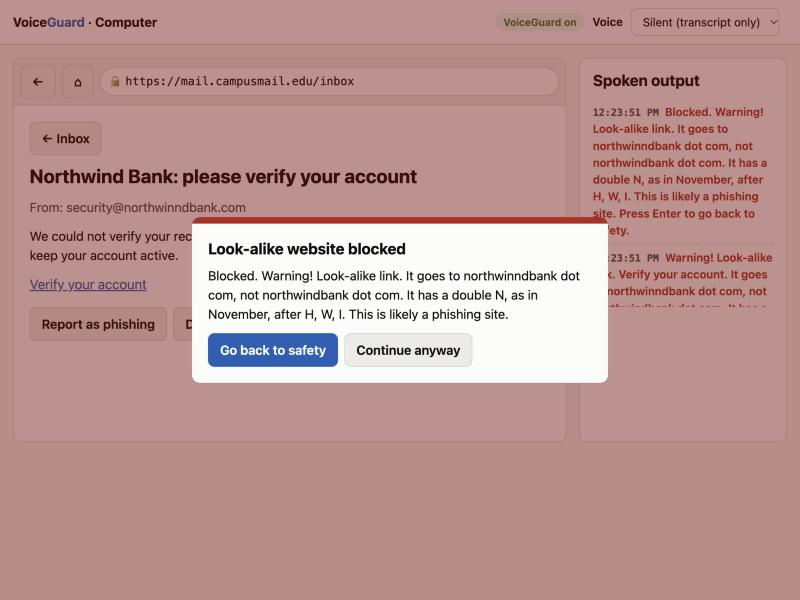
\includegraphics[width=\columnwidth]{figures/fig1-phishing-blocked.jpg}
\caption{The look-alike link \dom{northwinndbank.com} is blocked before the page loads. The spoken-output panel shows what the user hears, including the exact difference (``a double N, as in November'').}
\label{fig:phish}
\end{figure}

\subsection{Push Guard (P2, P3)}

\begin{itemize}
\item \textbf{No override.} Every waiting request stays listed and counted (``request 2 of 2''), each under its own heading, read oldest first. Focus moves to the new request's heading, never onto Approve.
\item \textbf{Spoken context.} Service, device, city and age of each request.
\item \textbf{Spoken code word.} On sign-in the computer says the code word twice; each push speaks its own, and no two waiting requests share one. An attacker who copies the victim's device and city still cannot know it (Fig.~\ref{fig:concurrent}).
\item \textbf{Concurrency alert} when more than one request is waiting.
\item \textbf{Fatigue lock.} Three requests within 2 minutes, or two refused or missed within 10 minutes, triggers a spoken warning and locks Approve for 5 minutes; the server enforces it (Fig.~\ref{fig:fatigue}).
\item \textbf{Adaptive expiry.} Long enough to hear the request twice plus 30\,s, never under 60\,s, with a ``15 seconds left'' cue.
\end{itemize}

\begin{figure}[t]
\centering
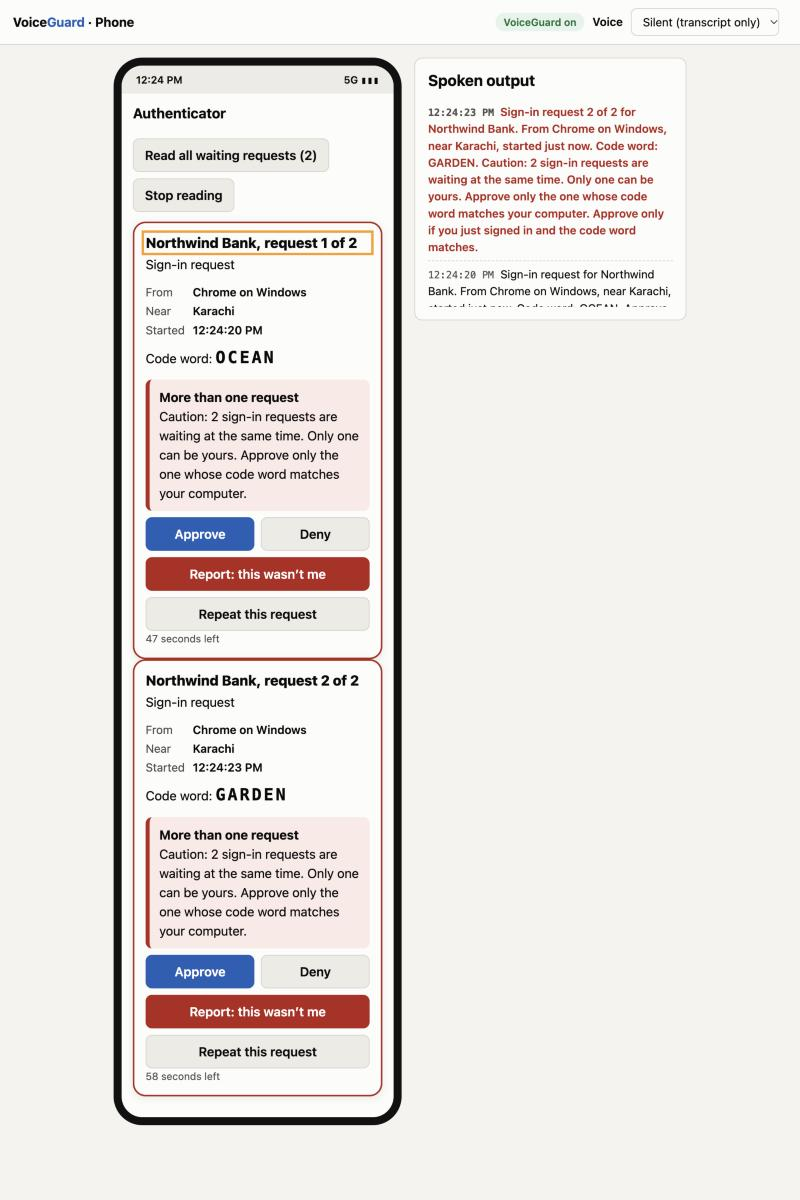
\includegraphics[width=\columnwidth]{figures/fig2-concurrent-code-words.jpg}
\caption{A concurrent-login race with a copied device. Both requests stay on the phone and both say ``Chrome on Windows, near Karachi''; only the code words differ.}
\label{fig:concurrent}
\end{figure}

\subsection{Voice Answers}

After a request is read, the phone beeps and listens. With VoiceGuard on, the user approves by saying ``approve'' plus the code word (``approve falcon''); ``yes'' alone is refused with a prompt to say the word, so the spoken answer is itself the code-word check. ``Deny'' and ``report'' act on the request; Baseline accepts ``yes'' and ``no''. The phone repeats what it heard. Because announcements contain the word ``approve'', the phone listens only after its own speech ends and ignores any phrase repeating five or more words it just said. A button remains as a fallback. Recognition uses the browser's speech service, which requires HTTPS.

\subsection{HCI Principles}

VoiceGuard applies \emph{visibility of system status} (every request listed; the real domain announced), \emph{error prevention} (fakes blocked; Approve locked under spam), \emph{match with the mental model} (the code word ties a push to the user's own sign-in), \emph{recognition over recall} (naming the difference instead of comparing spellings from memory) and \emph{accessibility of time} (expiry adapts to speech).

%======================================================================
\section{Implementation}

VoiceGuard is a dependency-free Node.js web application with 17 passing unit tests. It provides a simulated browser (mail, bank and payment sign-in, look-alike clones, and a log of everything spoken), a phone authenticator that runs on a real phone with VoiceOver or TalkBack, an attacker console, an experimenter console (participant and block, counterbalancing, six scripted tasks, automatic scoring, SUS~\cite{sus}, NASA-TLX~\cite{tlx} and trust ratings, CSV export), and a results page. Only fictional brands and a study password are used.

\emph{Baseline} reproduces today's behaviour as \emph{Broken Access} reports it: domains read as whole words, the newest push replacing the older one, no device details, and a change-password prompt after a denial. \emph{VoiceGuard} turns the protections on, each switchable for ablation. Announcements go to a built-in voice, to the participant's own screen reader through ARIA live regions, or both. If a password is typed on a fake page, the server immediately starts an attacker sign-in that sends a push, as real-time phishing kits do.

Recording the app's speech end to end exposed five problems; four were fixed (the look-alike warning spoken up to four times per link, a contradictory brand-in-subdomain message, the code word spoken three times in one breath, and a new-device warning repeated on every spam request). Baseline's misleading change-password step was kept on purpose, as it is the flaw the paper reports.

%======================================================================
\section{Evaluation Method}

We evaluate in four stages; only stage~4 involved a person.

\textbf{Stage 1: automated phishing evaluation.} From 50 frequently phished brands, including Pakistani ones (HBL, Meezan Bank, JazzCash, Easypaisa), we generated up to three look-alikes per technique: 1,114 fakes. Negatives were 85 legitimate sites not on the trusted list. A fake counts as detected only if VoiceGuard flags it and names the correct real site. Following AWARE, we rendered what the listener hears for the real and fake link, today and with VoiceGuard, normalised spellings a speech engine pronounces alike, and computed TF-IDF cosine similarity over character trigrams. Listening cost is speaking time at 180 words per minute.

\textbf{Stage 2: push-guard replay and ablation.} We replayed 7 concurrent-login races (attacker 0--60\,s after the victim), each with and without a spoofed device; 12 fatigue schedules (one push every 5\,s to 5\,min, denied or ignored); expiry at five speech rates; and normal sign-ins as negatives. For the ablation we switched off each component in turn and replayed the same scenarios.

\textbf{Stage 3: scripted end-to-end sessions.} A Playwright script drove the unmodified app in Chrome keyboard-only (Tab, Enter, typing), once per condition, through the six study tasks (Table~\ref{tab:tasks}) with the same brands and order. Announcements went to ARIA live regions and were captured from the app's spoken-output panel; the app scored each task. The scripted user approved only a request tied to its own sign-in, and in VoiceGuard only if the code word matched. This is an engineering check, not a user study.

\textbf{Stage 4: pilot with a blind participant.} One blind screen-reader user (P01) followed the planned within-subjects protocol: Baseline and VoiceGuard in counterbalanced blocks of the six tasks, Baseline first. P01 used a screen reader on the computer and a phone with its screen reader over a hotspot, and was told the study was about ``how easy it is to sign in with a screen reader''. Voice answering was added during the session, after the first fatigue task. Attempts that failed for technical reasons were excluded.

\begin{table}[t]
\caption{Study tasks (per block)}
\label{tab:tasks}
\footnotesize
\begin{tabularx}{\columnwidth}{@{}p{1.75cm}X@{}}
\toprule
Task & What happens (attack succeeds if) \\
\midrule
legit\_email & Real statement email, then sign in \\
legit\_login & Sign in to the payment app from a bookmark \\
phish\_typo & Email links to a doubled-letter look-alike (password typed on it) \\
phish\_subdomain & Email links to \dom{brand.com.account-verify.net} (password typed on it) \\
concurrent & Attacker signs in 2.5\,s after the user, copied device (attacker's push approved) \\
fatigue & Told not to sign in; 6 attacker pushes, 10\,s apart (any approved) \\
\bottomrule
\end{tabularx}
\end{table}

%======================================================================
\section{Data Collection}

Table~\ref{tab:data} lists everything collected. \textbf{One human participant} took part (P01, blind, daily screen-reader user). The scripted user in stage~3 is a program, not a participant. All other data come from generated stimuli and replayed attack schedules.

\begin{table*}[t]
\caption{Data collected in each stage}
\label{tab:data}
\centering
\footnotesize
\begin{tabularx}{\textwidth}{@{}p{3.2cm}p{4.6cm}X@{}}
\toprule
Stage & Amount & What was recorded \\
\midrule
1 Automated phishing & 1,114 look-alikes of 50 brands (9 techniques); 85 legitimate sites & Detection verdict and named target; spoken rendering today and with VoiceGuard; TF-IDF similarity; speaking time \\
2 Push replay and ablation & 7 races $\times$ 2 device conditions; 12 fatigue schedules; 5 speech rates; normal sign-ins; 8 configurations & Pushes shown, warnings raised, Approve lock, whether the two pushes sound different, expiry window \\
3 Scripted sessions & 1 scripted user $\times$ 2 conditions $\times$ 6 tasks = 12 task runs & Every announcement (spoken-output transcript), focus moves, actions, app-scored outcome per task \\
4 Pilot & 1 blind participant; 7 task attempts in the Baseline block, 2 valid and 5 excluded & Time-stamped event log (sign-ins, pushes, decisions, voice commands), app-scored outcome, decision time, observer notes \\
\midrule
\multicolumn{3}{@{}l}{\emph{Not collected:} the pilot's VoiceGuard block, SUS, NASA-TLX and trust questionnaires, and the debrief interview.} \\
\bottomrule
\end{tabularx}
\end{table*}

%======================================================================
\section{Results}

\subsection{Phishing: Fakes Become Audibly Different}

VoiceGuard detected 99.6\% of fakes (1,110 of 1,114), naming the correct real site each time, with 0\% false alarms (0 of 85). It reproduces the paper's finding: \dom{bankofamerica}/\dom{bankoffamerica} sounds 100\% identical today and 60.4\% similar with VoiceGuard; \dom{wellsfargo}/\dom{wellssfargo} goes from 100\% to 59.4\%. Today 21.4\% of all fakes sound identical to the real site, including 98.4\% of doubled-letter fakes and all Unicode look-alikes; with VoiceGuard none do. Mean similarity falls from 68.8\% to 49.1\% (Fig.~\ref{fig:similarity}).

\begin{figure}[t]
\centering
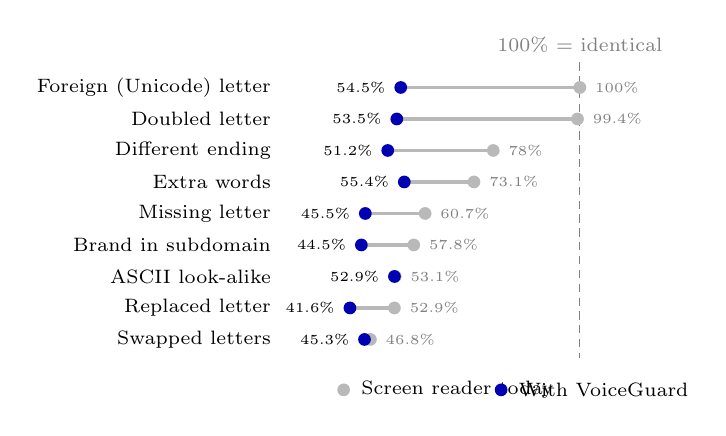
\begin{tikzpicture}[x=0.05cm,y=-0.4cm,font=\scriptsize]
\draw[densely dashed,gray] (100,-0.8) -- (100,8.6);
\node[gray,anchor=south] at (100,-0.8) {100\% = identical};
\foreach \n/\t/\g [count=\i from 0] in {
  Foreign (Unicode) letter/100/54.5,
  Doubled letter/99.4/53.5,
  Different ending/78/51.2,
  Extra words/73.1/55.4,
  Missing letter/60.7/45.5,
  Brand in subdomain/57.8/44.5,
  ASCII look-alike/53.1/52.9,
  Replaced letter/52.9/41.6,
  Swapped letters/46.8/45.3} {
  \draw[gray!55,line width=1.2pt] (\g,\i) -- (\t,\i);
  \fill[gray!55] (\t,\i) circle (2.3pt);
  \fill[blue!70!black] (\g,\i) circle (2.3pt);
  \node[anchor=east] at (24,\i) {\n};
  \node[anchor=west,gray,font=\tiny] at ([xshift=2pt]\t,\i) {\t\%};
  \node[anchor=east,font=\tiny] at ([xshift=-2pt]\g,\i) {\g\%};
}
\fill[gray!55] (40,9.6) circle (2.3pt); \node[anchor=west] at (42,9.6) {Screen reader today};
\fill[blue!70!black] (80,9.6) circle (2.3pt); \node[anchor=west] at (82,9.6) {With VoiceGuard};
\end{tikzpicture}
\caption{Spoken similarity to the real site (TF-IDF cosine, mean per technique, 1,114 fakes). The two techniques that sound identical today fall to about 55\% with VoiceGuard.}
\label{fig:similarity}
\end{figure}

The four misses were one-letter changes to the three-letter brand \dom{hbl.com}; names of three letters or fewer are deliberately not checked for single-letter typos, to avoid false alarms. The difference sentence takes 3.8\,s to hear on average, against 5.0\,s to spell the whole address, and spelling still leaves the comparison to memory. The full warning takes 10.4\,s, with the critical words first.

\subsection{Push Abuse: Every Replayed Attack Is Caught}

All eight push-guard checks passed. In every race from 0 to 60\,s, Baseline leaves only the attacker's push on the phone; VoiceGuard shows both and warns. When the attacker copies the victim's device and city, the spoken context can no longer separate the pushes, but the code word can. Under spam at any interval from 5\,s to 5\,min, the warning and Approve lock arrive by the third push. A single sign-in or a retry after a timeout raises no warning. Adaptive expiry gives 68\,s at the default rate (19\,s of speech) and 81\,s at 0.75$\times$ (25.3\,s). One push every 15 minutes is not detected.

\begin{figure}[t]
\centering
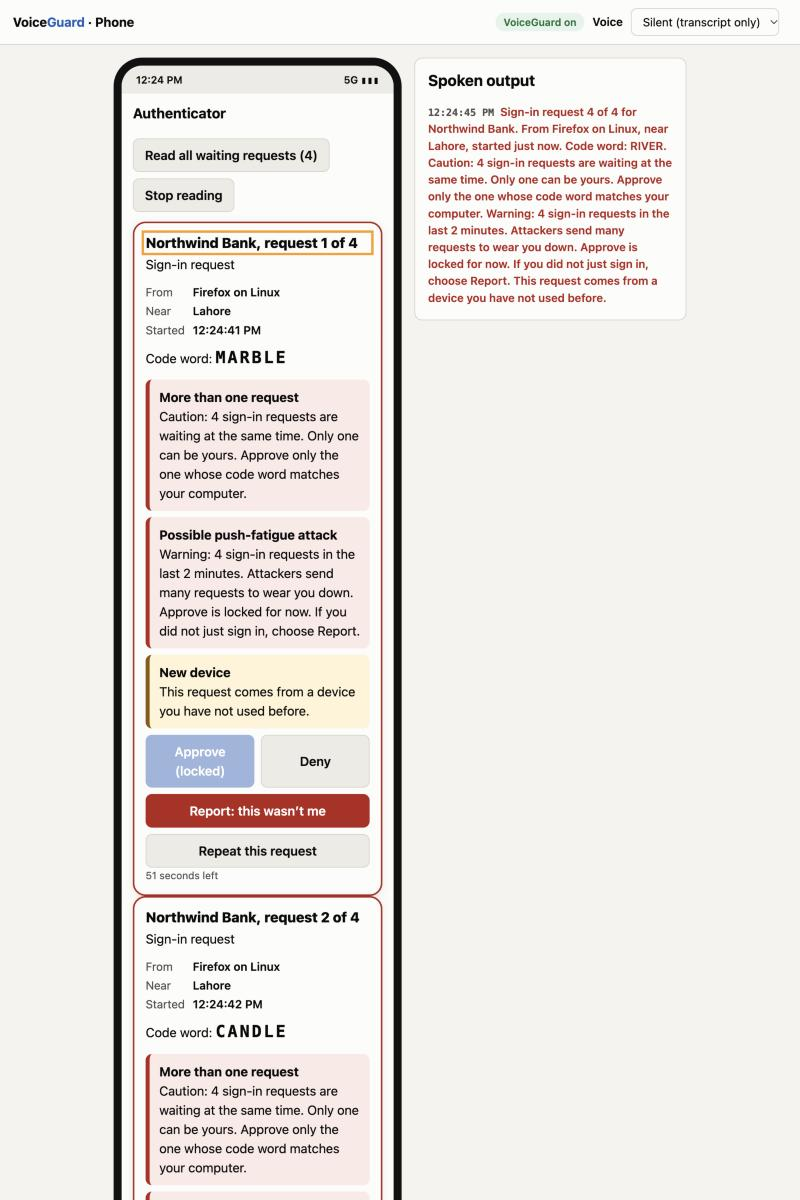
\includegraphics[width=\columnwidth]{figures/fig3-fatigue-locked.jpg}
\caption{Push spam. From the third request in two minutes, every request carries the fatigue warning and Approve is locked; Deny and Report stay available.}
\label{fig:fatigue}
\end{figure}

\subsection{Ablation: Each Protection Closes a Different Gap}

Table~\ref{tab:ablation} shows that once the device is spoofed, the code word is the only component that keeps the two pushes distinct, and the fatigue lock the only one that stops approval under spam. No configuration raised a false alarm on normal sign-ins.

\begin{table*}[t]
\caption{Push-guard ablation (7 races, 12 fatigue schedules)}
\label{tab:ablation}
\centering
\footnotesize
\begin{tabular}{@{}lccccc@{}}
\toprule
Configuration & Spoofed device: pushes sound different & Other device: new-device warning & Second request warned & Approve locked by 3rd spam push & Expiry at 1.0$\times$ / 0.75$\times$ \\
\midrule
Full VoiceGuard & 7/7 & 7/7 & 7/7 & 12/12 & 68\,s / 81\,s \\
Without context & 7/7 & 0/7 & 7/7 & 12/12 & 62\,s / 73\,s \\
Without code word & \textbf{0/7} & 7/7 & 7/7 & 12/12 & 60\,s / 69\,s \\
Without concurrency alert & 7/7 & 7/7 & \textbf{0/7} & 12/12 & 60\,s / 60\,s \\
Without fatigue lock & 7/7 & 7/7 & 7/7 & \textbf{0/12} & 68\,s / 81\,s \\
Without adaptive expiry & 7/7 & 7/7 & 7/7 & 12/12 & 60\,s / 60\,s \\
All off & 0/7 & 0/7 & 0/7 & 0/12 & 60\,s / 60\,s \\
\bottomrule
\end{tabular}
\end{table*}

\subsection{Scripted End-to-End Sessions}

Attacks succeeded 3 of 4 times in Baseline and 0 of 4 with VoiceGuard, and both legitimate sign-ins succeeded in both conditions (Table~\ref{tab:scripted}). In Baseline the fake link was read as ``northwiindbank dot com'' and the fake page sounded exactly like the real one; with VoiceGuard the user heard \say{It has a double I, as in India, after T, H, W.} Baseline fatigue was resisted only because the script denies any request it cannot tie to its own sign-in; its denial message (\say{Denied. Secure your account. Change password.}) was followed ten seconds later by an identical request, which would mislead a person.

\begin{table}[t]
\caption{Scripted keyboard-only sessions}
\label{tab:scripted}
\footnotesize
\begin{tabularx}{\columnwidth}{@{}p{1.75cm}XX@{}}
\toprule
Task & Baseline & VoiceGuard \\
\midrule
legit\_email & Signed in & Signed in \\
legit\_login & Signed in & Signed in \\
phish\_typo & \textbf{Attack succeeded} & Resisted, reported \\
phish\_subdomain & \textbf{Attack succeeded} & Resisted, reported \\
concurrent & \textbf{Attack succeeded} & Approved own, reported attacker's \\
fatigue & Resisted & Resisted; Approve locked \\
\bottomrule
\end{tabularx}
\end{table}

\subsection{Pilot With a Blind Participant}

P01 completed part of the Baseline block, and two tasks gave valid results. \textbf{Push fatigue: the attack succeeded.} After the sixth spam request, P01 pressed the voice button and said \say{Yes, I'm trying to sign in}, 44\,s after that request arrived, although they had been told not to sign in. \textbf{Legitimate sign-in: failed.} In 10 minutes P01 did not reach the payment app's bookmark; moving around an unfamiliar page by keyboard was itself a barrier.

Five attempts were excluded: two phishing attempts interrupted by setup changes (in one, the participant typed the password on the fake site and approved the relay push before the task was stopped), and three concurrent-login attempts in which no attack was delivered because the sign-in was not completed or the phone page had disconnected. The VoiceGuard block was not reached. Voice recognition worked on the participant's own phone.

%======================================================================
\section{Discussion}

\textbf{Audibility, not detection, is the gap.} Detecting look-alikes is a solved problem; what was missing is a way to \emph{say} the result so a listener can act on it. Naming the exact difference turns a 100\% audio match into a clearly different message, and the two techniques inaudible today gain the most.

\textbf{For push attacks, interface behaviour beats more information.} Device and city help only until the attacker copies them, and a newer push can bury an older one. Once the device is spoofed, only the code word separates the requests.

\textbf{Protection must act, not only warn.} P01 approved the sixth spam request while saying \say{Yes, I'm trying to sign in}. That is the moment the fatigue lock is built for: from the third request, giving in is no longer an option.

\textbf{Voice answers need guardrails.} A bare ``yes'' approves an attacker's request as easily as the user's own; requiring ``approve'' plus the code word makes the answer itself the check. A phone that listens on its own must also never hear itself.

\textbf{Running studies with blind participants is its own design problem.} The pilot lost most attack tasks to logistics: a phone that locked and disconnected, campus Wi-Fi that isolated devices, a screen reader not yet on, and unfamiliar keyboard navigation. A full study needs participants' own devices, auto-lock disabled, a private network and a longer familiarisation.

\textbf{Trade-offs.} Announcements are longer (about 10\,s for a link warning, 19\,s for a push), so critical words come first and the full warning is spoken once per link. The fatigue lock also blocks a genuine user who denies twice by mistake. In deployment, VoiceGuard would be split between a screen-reader add-on (domain warnings) and the service provider (no-override pushes and code words).

%======================================================================
\section{Limitations}

\begin{itemize}
\item \textbf{One human participant, one condition.} The pilot shows the attacks are real for a screen-reader user but cannot show that VoiceGuard helps people; a study with 20 participants is needed.
\item \textbf{Scripted end-to-end user.} It confirms that the mechanisms fire and the wording is right, not that people understand the NATO spelling or compare code words; its timings are machine timings.
\item \textbf{Modelled speech.} Similarity scores come from a model of screen-reader output, not recordings of real screen readers.
\item \textbf{Voice answering is partly tested.} A pressed-button voice answer worked on a real phone; automatic listening and its echo filter were tested only with simulated recognition results.
\item \textbf{Known gaps.} Three-letter brands get no typo checks, one push every 15 minutes evades the fatigue rules, and a copied device leaves only the code word.
\item \textbf{Setting.} A high attack base rate, fictional brands, and speech output only (no braille displays).
\end{itemize}

%======================================================================
\section{Ethics}

The pilot participant gave verbal informed consent, was told they could stop at any time and withdraw their data, and was not warned about attacks in advance. No formal ethics approval was obtained for this course project; a full study would need it. Only fictional brands and a study password were used, data are identified only by participant ID and kept out of the project repository, and voice recognition sends audio to the browser's speech service, which a full study must disclose.

%======================================================================
\section{Conclusion and Future Work}

\textbf{Were the objectives achieved?} Partly (Table~\ref{tab:achieved}). The system-level objectives were met: VoiceGuard makes all three attacks audible and stops them in automated and scripted tests (RQ1--RQ3, RQ5). The human-level objective was not: with one participant who did not reach the VoiceGuard block, we cannot yet show that VoiceGuard helps people or what it costs them in usability (RQ4).

\begin{table}[t]
\caption{Research questions and outcome}
\label{tab:achieved}
\footnotesize
\begin{tabularx}{\columnwidth}{@{}p{0.75cm}p{1.15cm}X@{}}
\toprule
RQ & Status & Evidence \\
\midrule
RQ1 & Partly & 99.6\% of fakes detected; scripted phishing 2/2 succeeded in Baseline, 0/2 with VoiceGuard; not tested with people \\
RQ2 & Partly & Every replayed race caught; code word separates spoofed pushes (ablation); scripted attack stopped; pilot attempts excluded \\
RQ3 & Partly & Approve locked by the 3rd push in 12/12 schedules; pilot confirms the problem (P01 approved the 6th spam push in Baseline); VoiceGuard not tested with people \\
RQ4 & Not yet & Scripted legitimate sign-ins succeed in both conditions; no human usability data \\
RQ5 & Achieved & 100\% to 60.4\% similarity for the paper's pair; fakes that sound identical fall from 21.4\% to 0\% (modelled speech) \\
\bottomrule
\end{tabularx}
\end{table}

\emph{Broken Access} showed that sign-in security fails screen-reader users through the audio channel. VoiceGuard shows this can be fixed by changing what is said: name exactly how a fake site differs, never let one push hide another, tie each push to the user's sign-in with a spoken code word, act on push spam instead of only warning, and give users time to listen. Our evaluation reproduces the paper's 100\% similarity finding and removes it, detecting 99.6\% of 1,114 fakes with no false alarms; the ablation shows each protection closes a distinct gap; end-to-end sessions show VoiceGuard stopping every attack that succeeded under today's behaviour without blocking normal sign-ins; and a pilot confirmed push fatigue on a real screen-reader user. Next steps are a counterbalanced study with 20 blind and visually impaired participants after ethics approval, replication with recorded screen-reader audio, an NVDA add-on for real browsing, and service-side support for no-override pushes and spoken code words.

Code, tests, evaluation scripts and session recordings: \url{https://github.com/abbyferoz/voiceguard-accessible-auth}.

%======================================================================
% References compiled from memory; check details before submission.
\begin{thebibliography}{8}

\bibitem{brokenaccess}
M.~A. Akanda, A.~T. Mahdad, and N.~Saxena, ``Broken Access: On the challenges of screen reader assisted two-factor and passwordless authentication,'' in \emph{Proc. ACM Web Conference (WWW '25)}, Sydney, Australia, 2025.

\bibitem{homograph}
E.~Gabrilovich and A.~Gontmakher, ``The homograph attack,'' \emph{Communications of the ACM}, vol.~45, no.~2, 2002.

\bibitem{typosquat}
J.~Szurdi, B.~Kocso, G.~Cseh, J.~Spring, M.~Felegyhazi, and C.~Kanich, ``The long `taile' of typosquatting domain names,'' in \emph{Proc. USENIX Security Symposium}, 2014.

\bibitem{combosquat}
P.~Kintis \emph{et~al.}, ``Hiding in plain sight: A longitudinal study of combosquatting abuse,'' in \emph{Proc. ACM CCS}, 2017.

\bibitem{tr39}
Unicode Consortium, ``Unicode Technical Standard \#39: Unicode Security Mechanisms.''

\bibitem{punycode}
A.~Costello, ``Punycode: A Bootstring encoding of Unicode for Internationalized Domain Names in Applications (IDNA),'' IETF RFC 3492, 2003.

\bibitem{sus}
J.~Brooke, ``SUS: A `quick and dirty' usability scale,'' in \emph{Usability Evaluation in Industry}, 1996.

\bibitem{tlx}
S.~G. Hart and L.~E. Staveland, ``Development of NASA-TLX (Task Load Index),'' \emph{Advances in Psychology}, vol.~52, 1988.

\end{thebibliography}

\end{document}
